\documentclass[11pt]{beamer}
\usetheme{Warsaw}
\usepackage[utf8]{inputenc}
\usepackage[english]{babel}
\usepackage{amsmath}
\usepackage{amsfonts}
\usepackage{amssymb}
\usepackage{color}
\usepackage{graphicx}
\definecolor{gray}{gray}{0.55}
\author{\textcolor{gray}{Adel Benamara} \and \underline{Thomas Gougeon} \and \underline{Ludovic
Robin}}
\title{Library version checking - QuarksLab}
%\setbeamercovered{transparent} 
%\setbeamertemplate{navigation symbols}{} 
%\logo{} 
%\institute{} 
%\date{} 
%\subject{} 
\begin{document}

\begin{frame}
\titlepage
\end{frame}

\begin{frame}
\tableofcontents
\end{frame}

\section{Introduction}
\begin{frame}{Introduction}

    \begin{center}
    
\includegraphics[scale=0.38]{hacker.png}
    \end{center}

    \begin{block}{}
        \begin{itemize}
            \item \underline{Hackers} look for vulnerabilities in programs ;
            \item Sometimes, finding one allow them to make an exploit ;
            \item \underline{Developers} try to fix vulnerabilities, publishing a patch ;
            \item \underline{Users} install the patch to hopefully fix the vulnerability on
                their version of the program.
        \end{itemize}
    \end{block}
\end{frame}

\begin{frame}
    \frametitle{What could go wrong ?}
    \begin{center}
    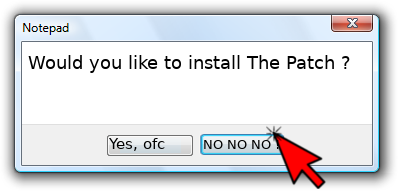
\includegraphics[scale=0.5]{box.png}
    \end{center}

    \begin{block}{}
    \begin{itemize}
        \item The vulnerability is not necessarily patched and the old version may remain ;
        \item \Huge Very \textcolor{red}{dangerous} !
    \end{itemize}
    \end{block}

    \end{frame}

\begin{frame}
    \frametitle{Use your hands} 
    \begin{block}{Strings}
        We use the strings command to check for infos in binary.
    \end{block}
    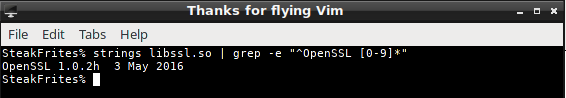
\includegraphics[scale=0.5]{strings.png}
    \begin{block}{Other methods}
       We do not know any... But pros do.
    \end{block}
    Is there any pro here ? 
\end{frame}


\begin{frame}
    \frametitle{Overview - How to check if we applied a patch ?}
   
    \begin{block}{What do we have ?}
        \begin{itemize}
            \item An unknown .so library, $L$ ;
            \item A set of known libraries sources, $S$.
        \end{itemize}
    \end{block}

    \begin{center}
        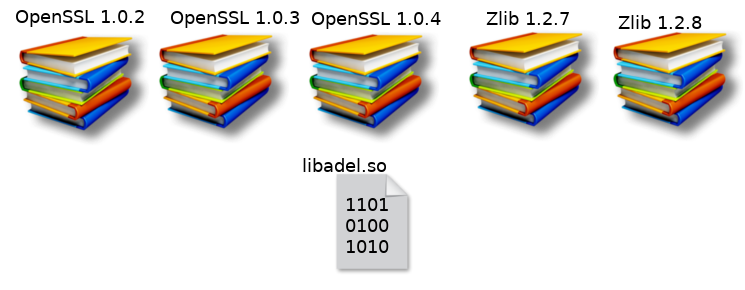
\includegraphics[scale=0.3]{bdd.png} 
    \end{center}

    \begin{block}{What are we doing ?}
        For all library $s$ in $S$, we check if $L$ is of the same version as $s$.
    \end{block}
\end{frame}


\begin{frame}
    \frametitle{Lazy start}

    
    \begin{block}{}
        \begin{itemize}
            \item Compile libraries in $S$, $c_1, \dots, c_n$ ; 
            \item Compare bit by bit $L$ and $c_1, \dots, c_n$.
        \end{itemize}
    \end{block}
    \begin{center}
    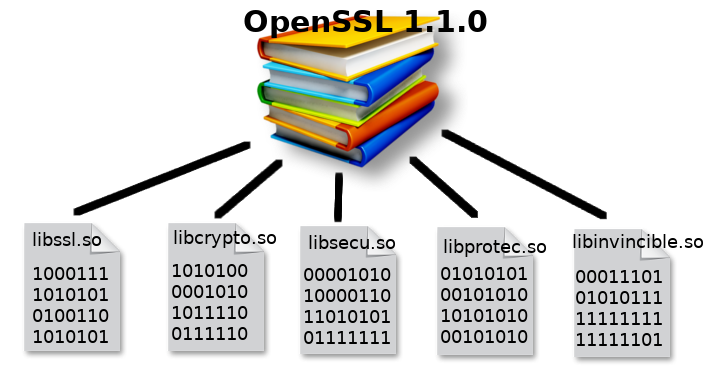
\includegraphics[scale=0.2]{compillib.png}
        \hspace{5em}
    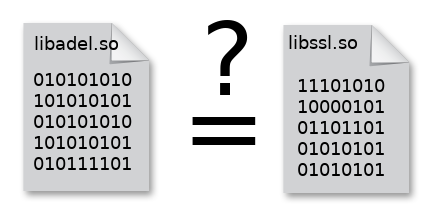
\includegraphics[scale=0.2]{compbin.png}
    \end{center}
    \begin{block}{}
        $L$ is compiled with a \underline{different compiler} and \underline{different
        compiling options}.
    \end{block}

\end{frame}

\begin{frame}
    \frametitle{Be smarter}

    \begin{block}{}
    \begin{itemize}
        \item Link compatibility ;
        \item Malware signature ;
        \item Traces.
    \end{itemize}
    \end{block}
    \begin{center}
        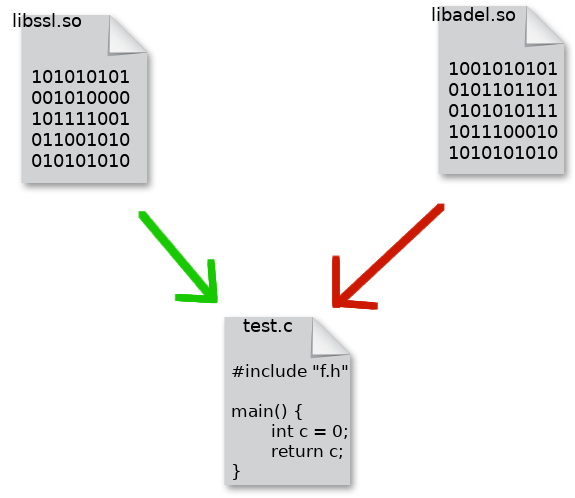
\includegraphics[scale=0.2]{link.png}
    
\includegraphics[scale=0.4]{malware.jpeg}
    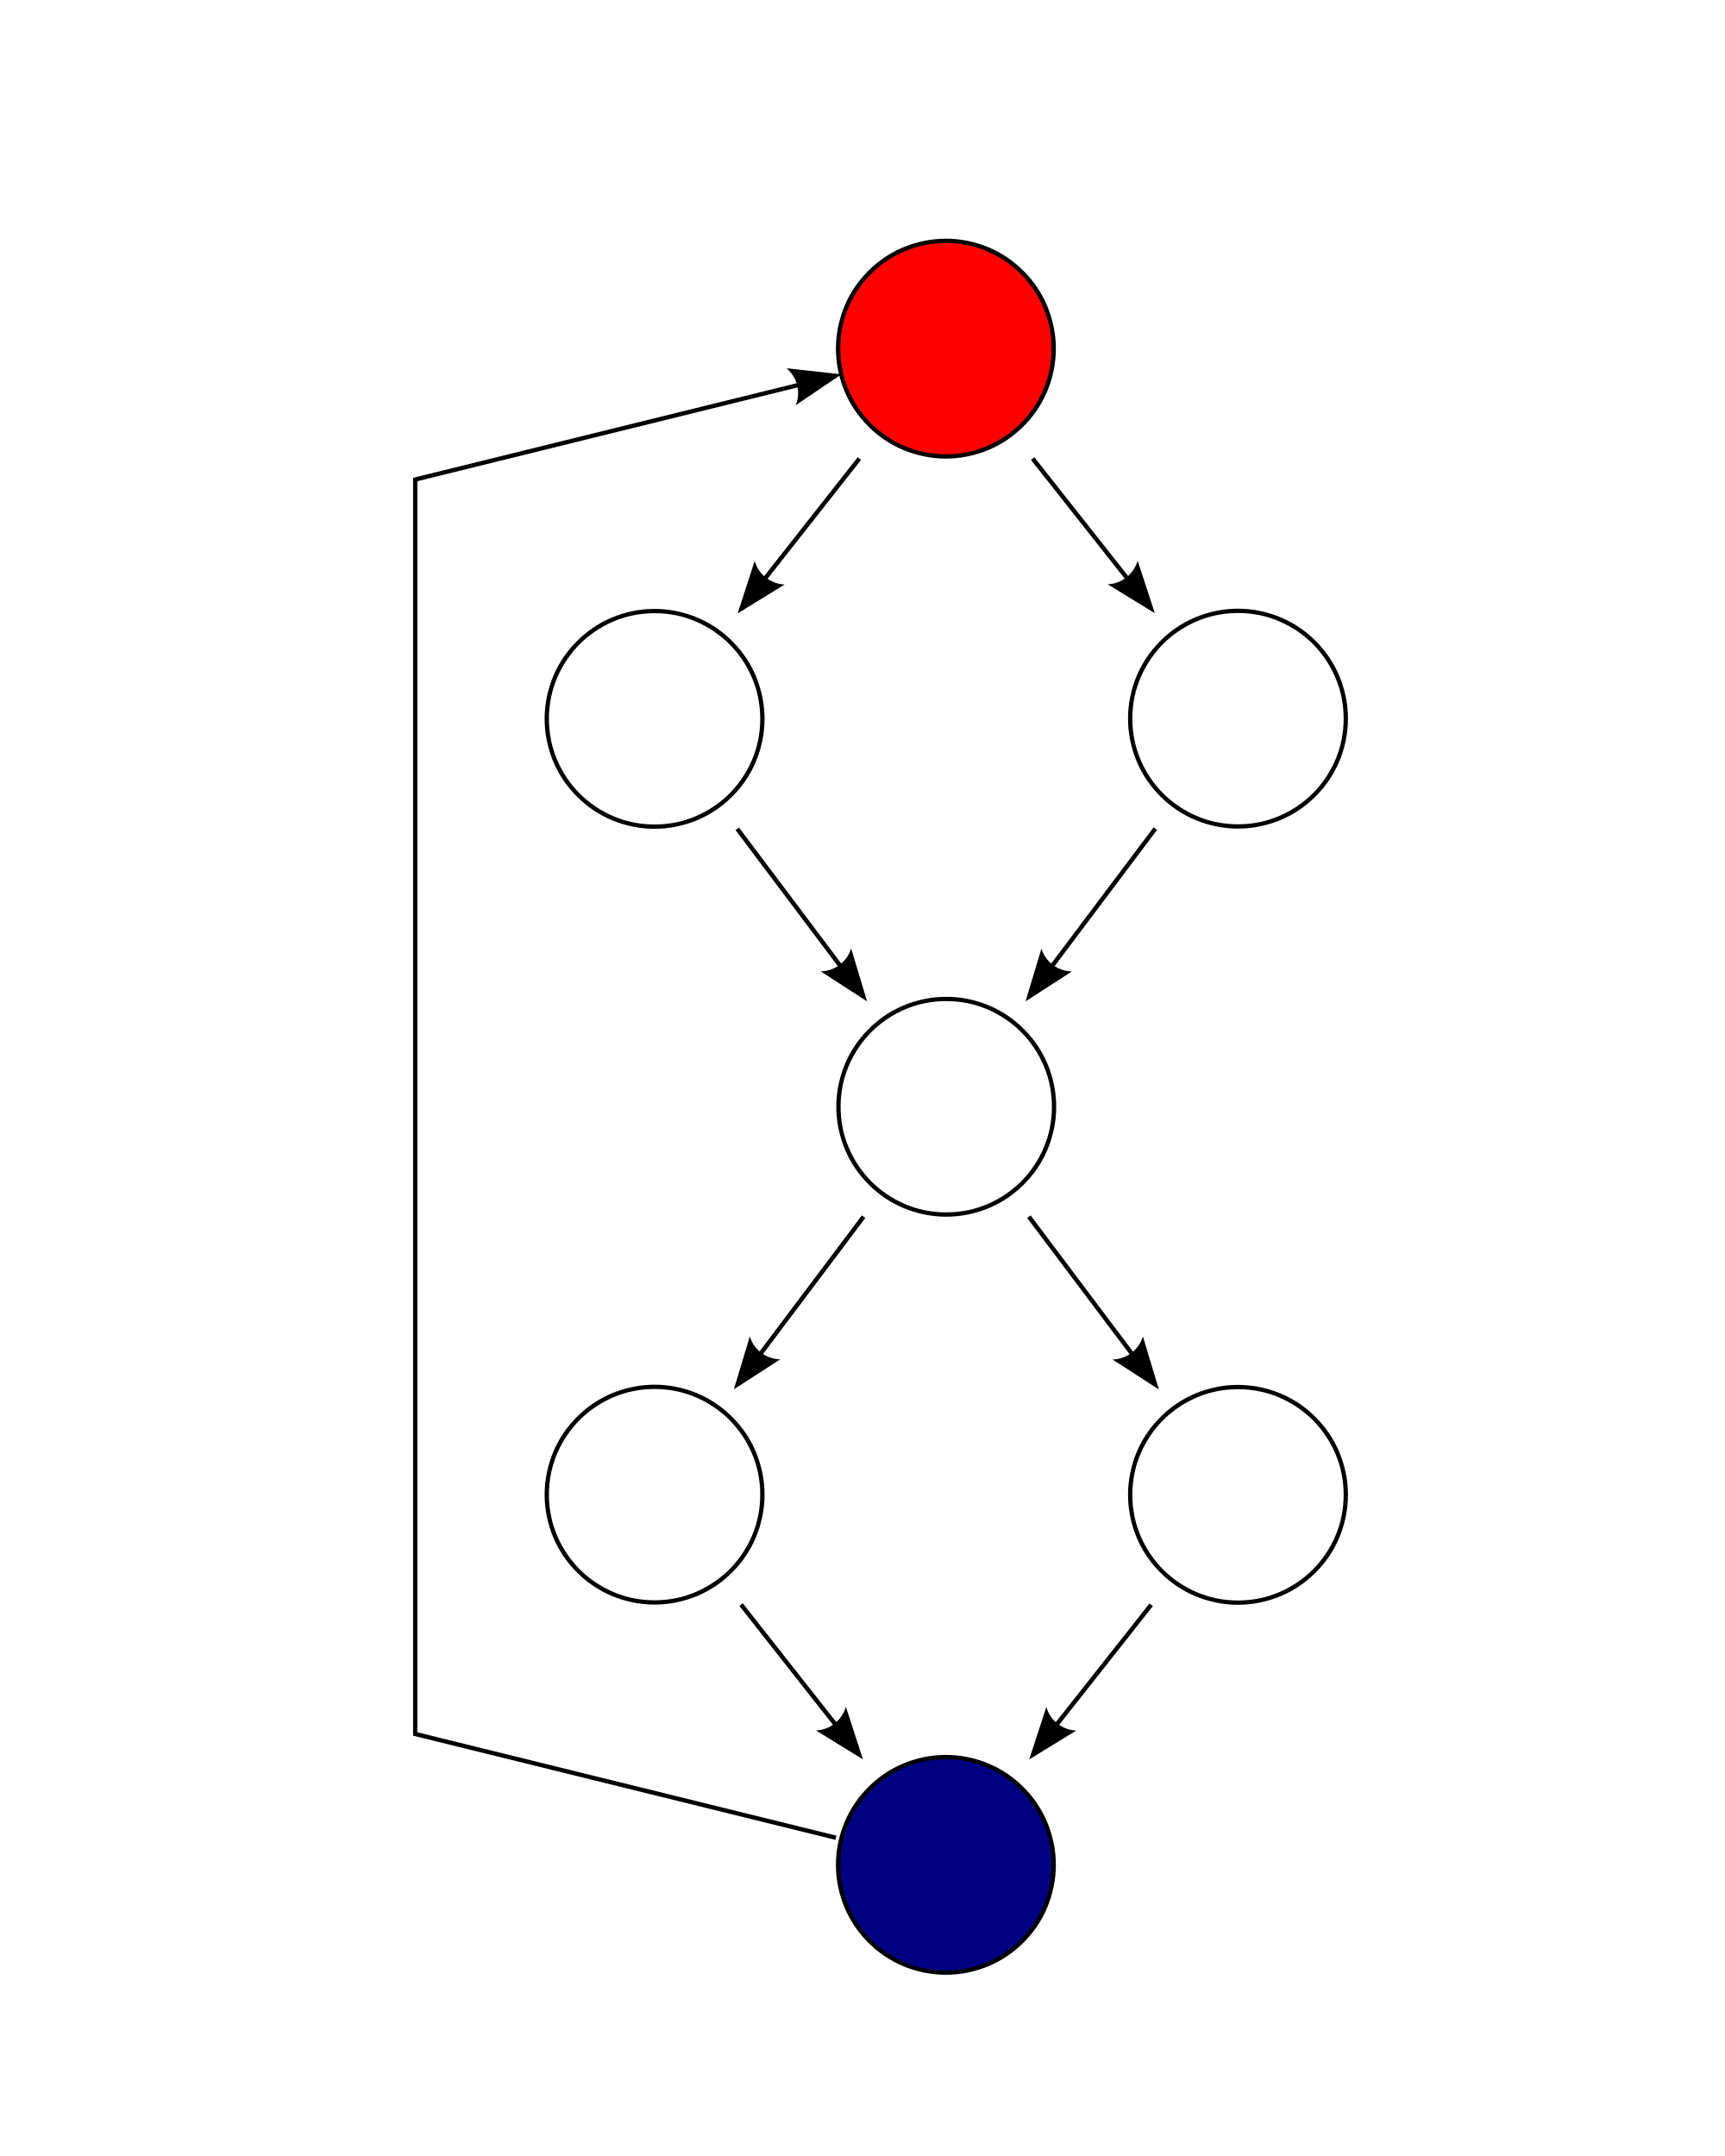
\includegraphics[scale=0.05]{cfg.png}
    \end{center}

\end{frame}

\begin{frame}
    \frametitle{Link dynamically the library}
    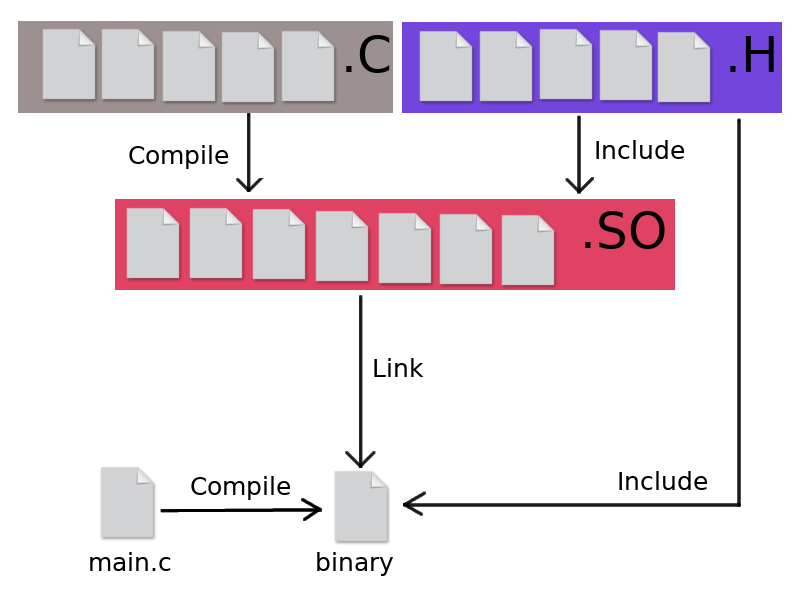
\includegraphics[scale=0.38]{compil1.png}
\end{frame}

\begin{frame}
    \frametitle{Link dynamically the library}
    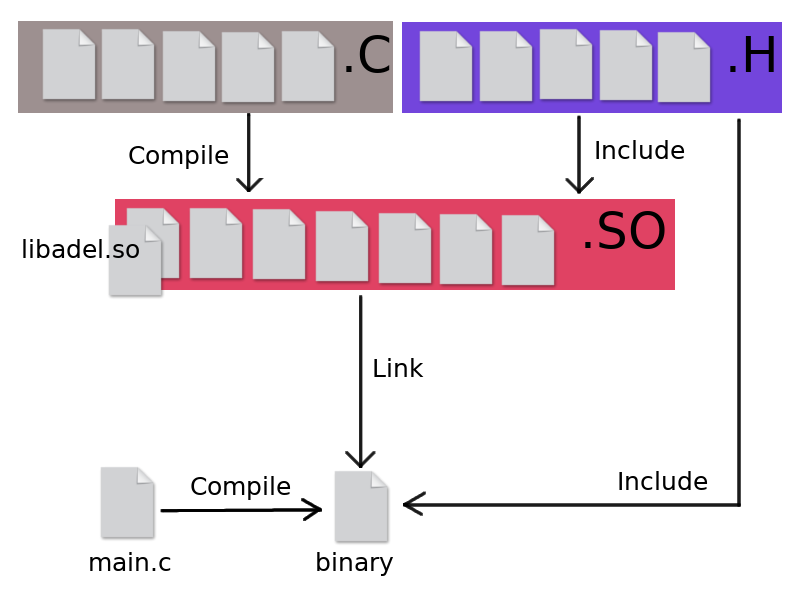
\includegraphics[scale=0.38]{compil2.png}
\end{frame}

\begin{frame}
    \frametitle{Turnkey programs} 
    \begin{block}{Build a DB}
        \begin{itemize}
            \item Semi-auto-compiling libraries ;
            \item Semi-auto-extracting headers ;
            \item Auto-generation of a c program to link-test libraries ;
        \end{itemize}
    \end{block}
    \begin{block}{Executable}
         \begin{itemize}
                \item Checking major version of a library with link-testing. 
         \end{itemize}
    \end{block}
    \begin{block}{Tested with OpenSSL 1.0.2h}
        \begin{itemize}
            \item OpenSSL 1.0.2j - cannot distinguish 
            \item OpenSSL 1.0.1e - can distinguish
        \end{itemize}
    \end{block}

\end{frame}

\begin{frame}
    \frametitle{Malware signature}
    
\end{frame}

\begin{frame}
    \frametitle{Analyse traces} 
\end{frame}


\begin{frame}{Tools that could be interesting, but are not.}

\begin{block}{Coccinelle}
	\begin{itemize}
		\item Find known bugs in source code
		\item Analyse patterns in source
		\item Issue: We deal with binaries
		\item Useful to find other execution paths for root cause
	\end{itemize}
\end{block}

\end{frame}



\section{Conclusion}


\begin{frame}{Conclusion}

	\begin{block}{Issues}
		\begin{itemize}
			\item Tools are too specific to some cases, not our cases.
		\end{itemize}
	\end{block}

	\begin{block}{Results}
		\begin{itemize}
			\item Differentiate major versions ;
            \item Some ideas to do better.
		\end{itemize}
	\end{block}
\end{frame}


\begin{frame}{It brought us..}


\begin{block}{Mind}
	\begin{itemize}
		\item Inner peace
		\item Happiness
        \item Intimacy
        \item We lost faith in formal methods, for binary analysis at least.
	\end{itemize}
\end{block}

\begin{block}{Technical}
	\begin{itemize}
        \item We got back our Perl, that is priceless.
		\item Binaries are complex but fun ;
	\end{itemize}
	
\end{block}

\end{frame}
\end{document}
